\chapter{Data measurement and analysis} \label{ch:data}

\vspace{-1.5 em}
\begin{addmargin}[-0.5cm]{0cm}
  \minitoc
\end{addmargin}
\hrule
\vspace{1.5 em}

\section{Data measurement and analysis}
The premise of CEI is simple enough for a quirky elevator pitch yet the collecton and analysis of data is a nuanced multi-step process as we are attempting to measure each single atomic fragment precisely. In this section we will go through the process of how the momentum vectors of each atomic fragment are measured. This will require some discussion regarding the apparatus, algorithms, and intricacies of the process, all of which are essential to understand exactly how the data is collected so that it can be analyzed appropriately. We will also quantify the uncertainty in those measurements, which will be essential in quantifying our uncertainty in the reconstructed geometries later on.

\subsection{Time and position measurement}
The time-of-flight of each atomic fragment and its position on the detector are required to calculate its momentum vector. The measurement of time and position is carried out by a two-stage apparatus feeding electrical signals into a data acquisition (DAQ) computer which analyzes the signals to determine time and position.

The first part of the two-stage apparatus is a set of two multi-channel plates (MCP) placed in a chevron configuration.\footnotemark~ Figure \ref{fig:MCP} shows a schematic of an MCP and briefly describes its operation. The job of the MCP is to amplify the signal of a single charged particle enough such that it may be detected as an electrical signal by an oscilloscope, much like a photomultiplier tube. Thus the output of an MCP is a shower of charged particles, or rather a charged cloud. The charged cloud may be fed into a second MCP to further amplify the signal. A two-stage chevron MCP setup produces an amplification of approximately $10^5-10^6$ depending on the applied voltage $V_D$ across the channels.

\footnotetext{The channels of an MCP are slanted, usually at a (bias) angle of $5\degree-15\degree$ to increase the probability that an incident particle collides with the channel wall. To further increase this probability, the second MCP is oriented such that its channels are slanted in the opposite direction forming a V-like (or chevron-like) channel configuration.}

\begin{SCfigure}
  \centering
  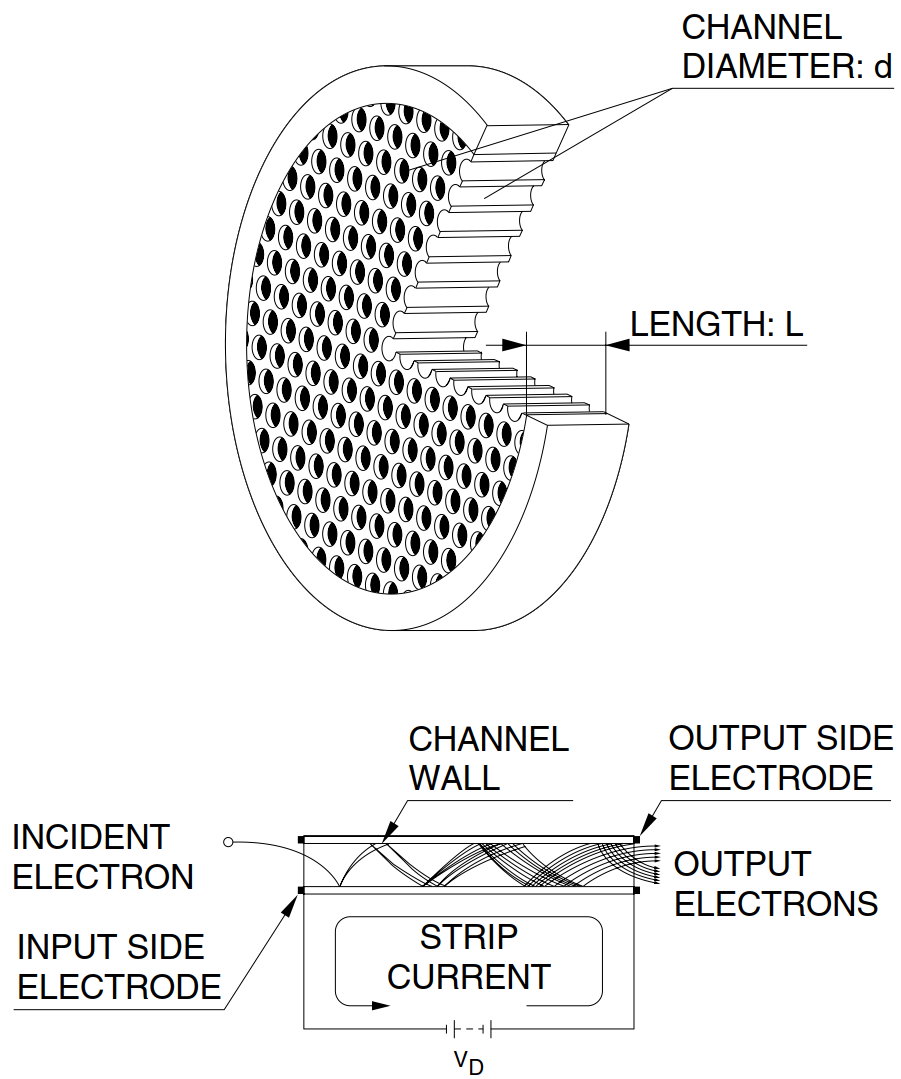
\includegraphics[width=0.50\textwidth]{gfx/MCP}
  \caption
  [Schematic of a multi-channel plate (MCP).]
  {Schematic of a multi-channel plate (MCP). The incident particle need not be an electron, and may in fact be any charged particle or even a high-energy photon. Once a charged particle is incident on an MCP and collides with a channel wall, multiple secondary electrons are emitted and accelerated up the channel due to the applied voltage $V_D$ setting up a potential gradient along the channel and replenishing the emitted electrons. Due to the angled channels, the emitted electrons follow parabolic trajectories hitting the other wall and continuing the amplification process until a large number of particles are emitted at channel output.}
  \label{fig:MCP}
\end{SCfigure}

You may notice that while most of the MCP's surface is covered in channels, not all of it is, leading to non-perfect detection. Only 60\% of the area is open to incident particles, and if a particle is incident on the other 40\% then it is not detected. Thus the detection efficiency of a triple coincidence event is $(0.6)^3 \approx 0.2$ and so we see that detection effiency decreases rapidly with the number of fragments that must be detected, suggesting that larger molecules are more difficult to study. There do exist ``funnel'' MCPs with an open area ratio of 90\% that increase the detection efficiency.

By itself this MCP setup is enough to provide time-of-flight information but to obtain position information, this charged cloud output is made incident on a ``modified backgammon with weighted capacitors'' anode or readout pad built as described by \citet{Veshapidze02}. Figure \ref{fig:MBWC} shows a schematic of such an anode and describes the position detection process.

\begin{figure}
  \centering
  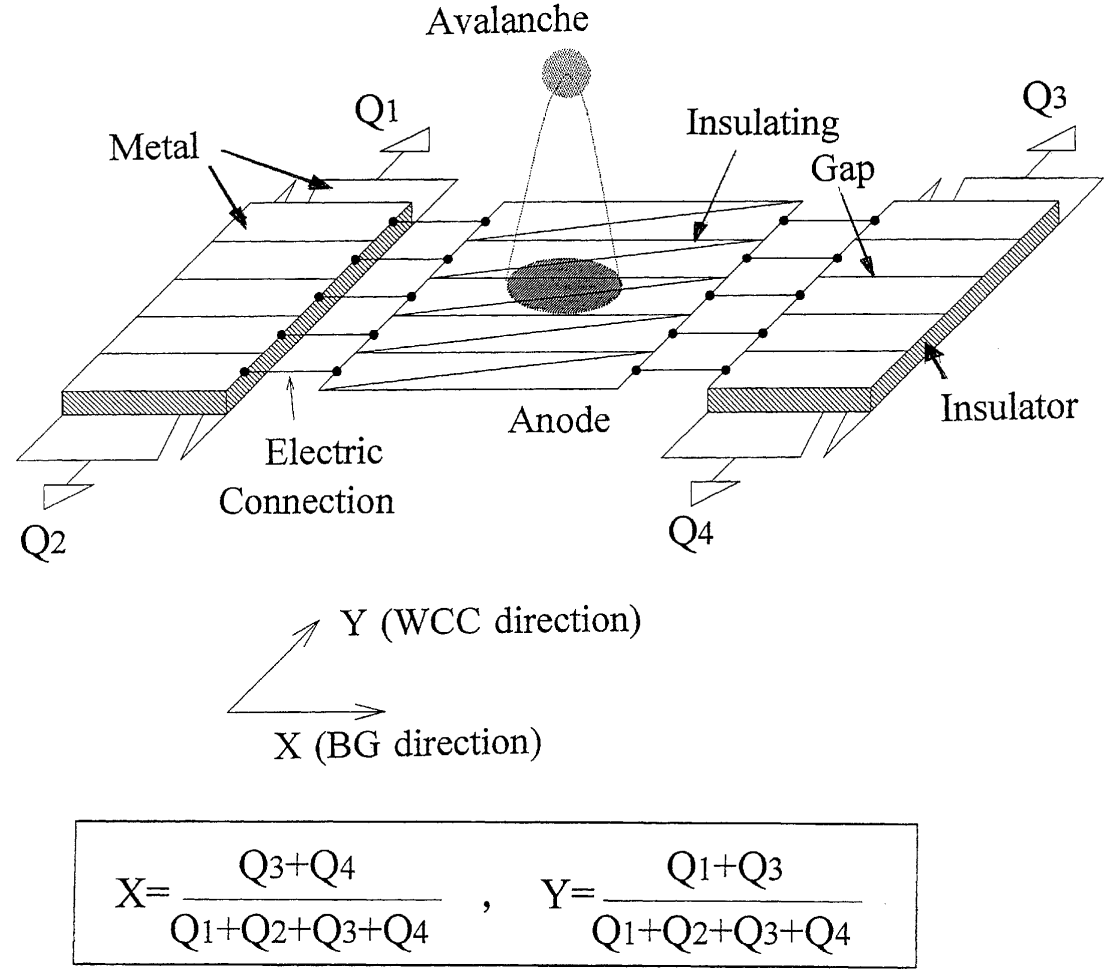
\includegraphics[width=\textwidth]{gfx/MBWC}
  \caption
  [Schematic of a symmetrized ``modified backgammon with weighted capacitors'' (MBWC) anode for position detection.]
  {Schematic of a symmetrized ``modified backgammon with weighted capacitors'' (MBWC) anode for position detection. The avalanche of charged particles or charged cloud hits the anode and induces a charge on the anode. This charged is induced via the capacitive couplings from the feedback capacitors of the preamplifiers connected to the triangles. The lines on the anode are insulating gaps, splitting the anode into a series of triangles whose arrangement resemble that of the backgammon board game. The metal strips are capacitively coupled to the triangluar strips through the insulator. If the cloud lands on the right side of the anode, then a larger fraction of the induced charge will flow to $Q_3$ and $Q_4$. So we can see that $x=0$ corresponds to the left side of the anode, and $x=1$ to the right side. If the cloud lands further up the anode, then a larger fraction of the induced charge will flow through $Q_1$ and $Q_3$ so we see that $y=0$ corresponds to the bottom side of the anode and $y=1$ corresponds to the top side. It is worth noting that the sign of $Q_i$ depends on the sign of the induced charge, and thus on the sign of the incident charged particle. In CEI the charged particles are all ions so $Q_i$ is always positive. The design gets its name as it is a combination of two older designs, the ``backgammon'' (BG) and the ``weighted coupling capacitor'' (WCC) designs. \citet{Mizogawa92} provides a more detailed explanation of its operation.  Figure rom \citet{Mizogawa02}. Reprinted with permission from Elsevier.}
  \label{fig:MBWC}
\end{figure}

These four signals are fed into an Ortec 142 preamplifier in energy output mode, essentially acting as an operational amplifier integrator. The integrated signal is then fed into a digital acquisition (DAQ) computer equipped with a four-channel oscilloscope. Every time a laser pulse is fired into the experiment, an electrical signal is sent to the oscilloscope as a trigger. The DAQ examines the four signals following a trigger and saves them if it sees evidence of charged particle detection.

A particularly good example of a triple coincidence detection event can be seen in figure \ref{fig:tripleCoincidence} along with an analysis of what can be gleaned about the Coulomb explosion process just by inspection of the signals on the oscilloscope. As a side note, if too many atomic fragments arrive at the detector in a short enough time period, steps due to different molecules may get mixed. Thus it is important to keep the Coulomb explosion rate low (\SI{100}{\Hz} worked quite well). Another reason to keep the count rate low is that the signals need time to decay back down post-integration otherwise the signals will saturate the oscilloscope at \SI{200}{\mV}. The ringing artifacts on the signal are due to the response of the preamplifiers.

\begin{figure}
  \centering
  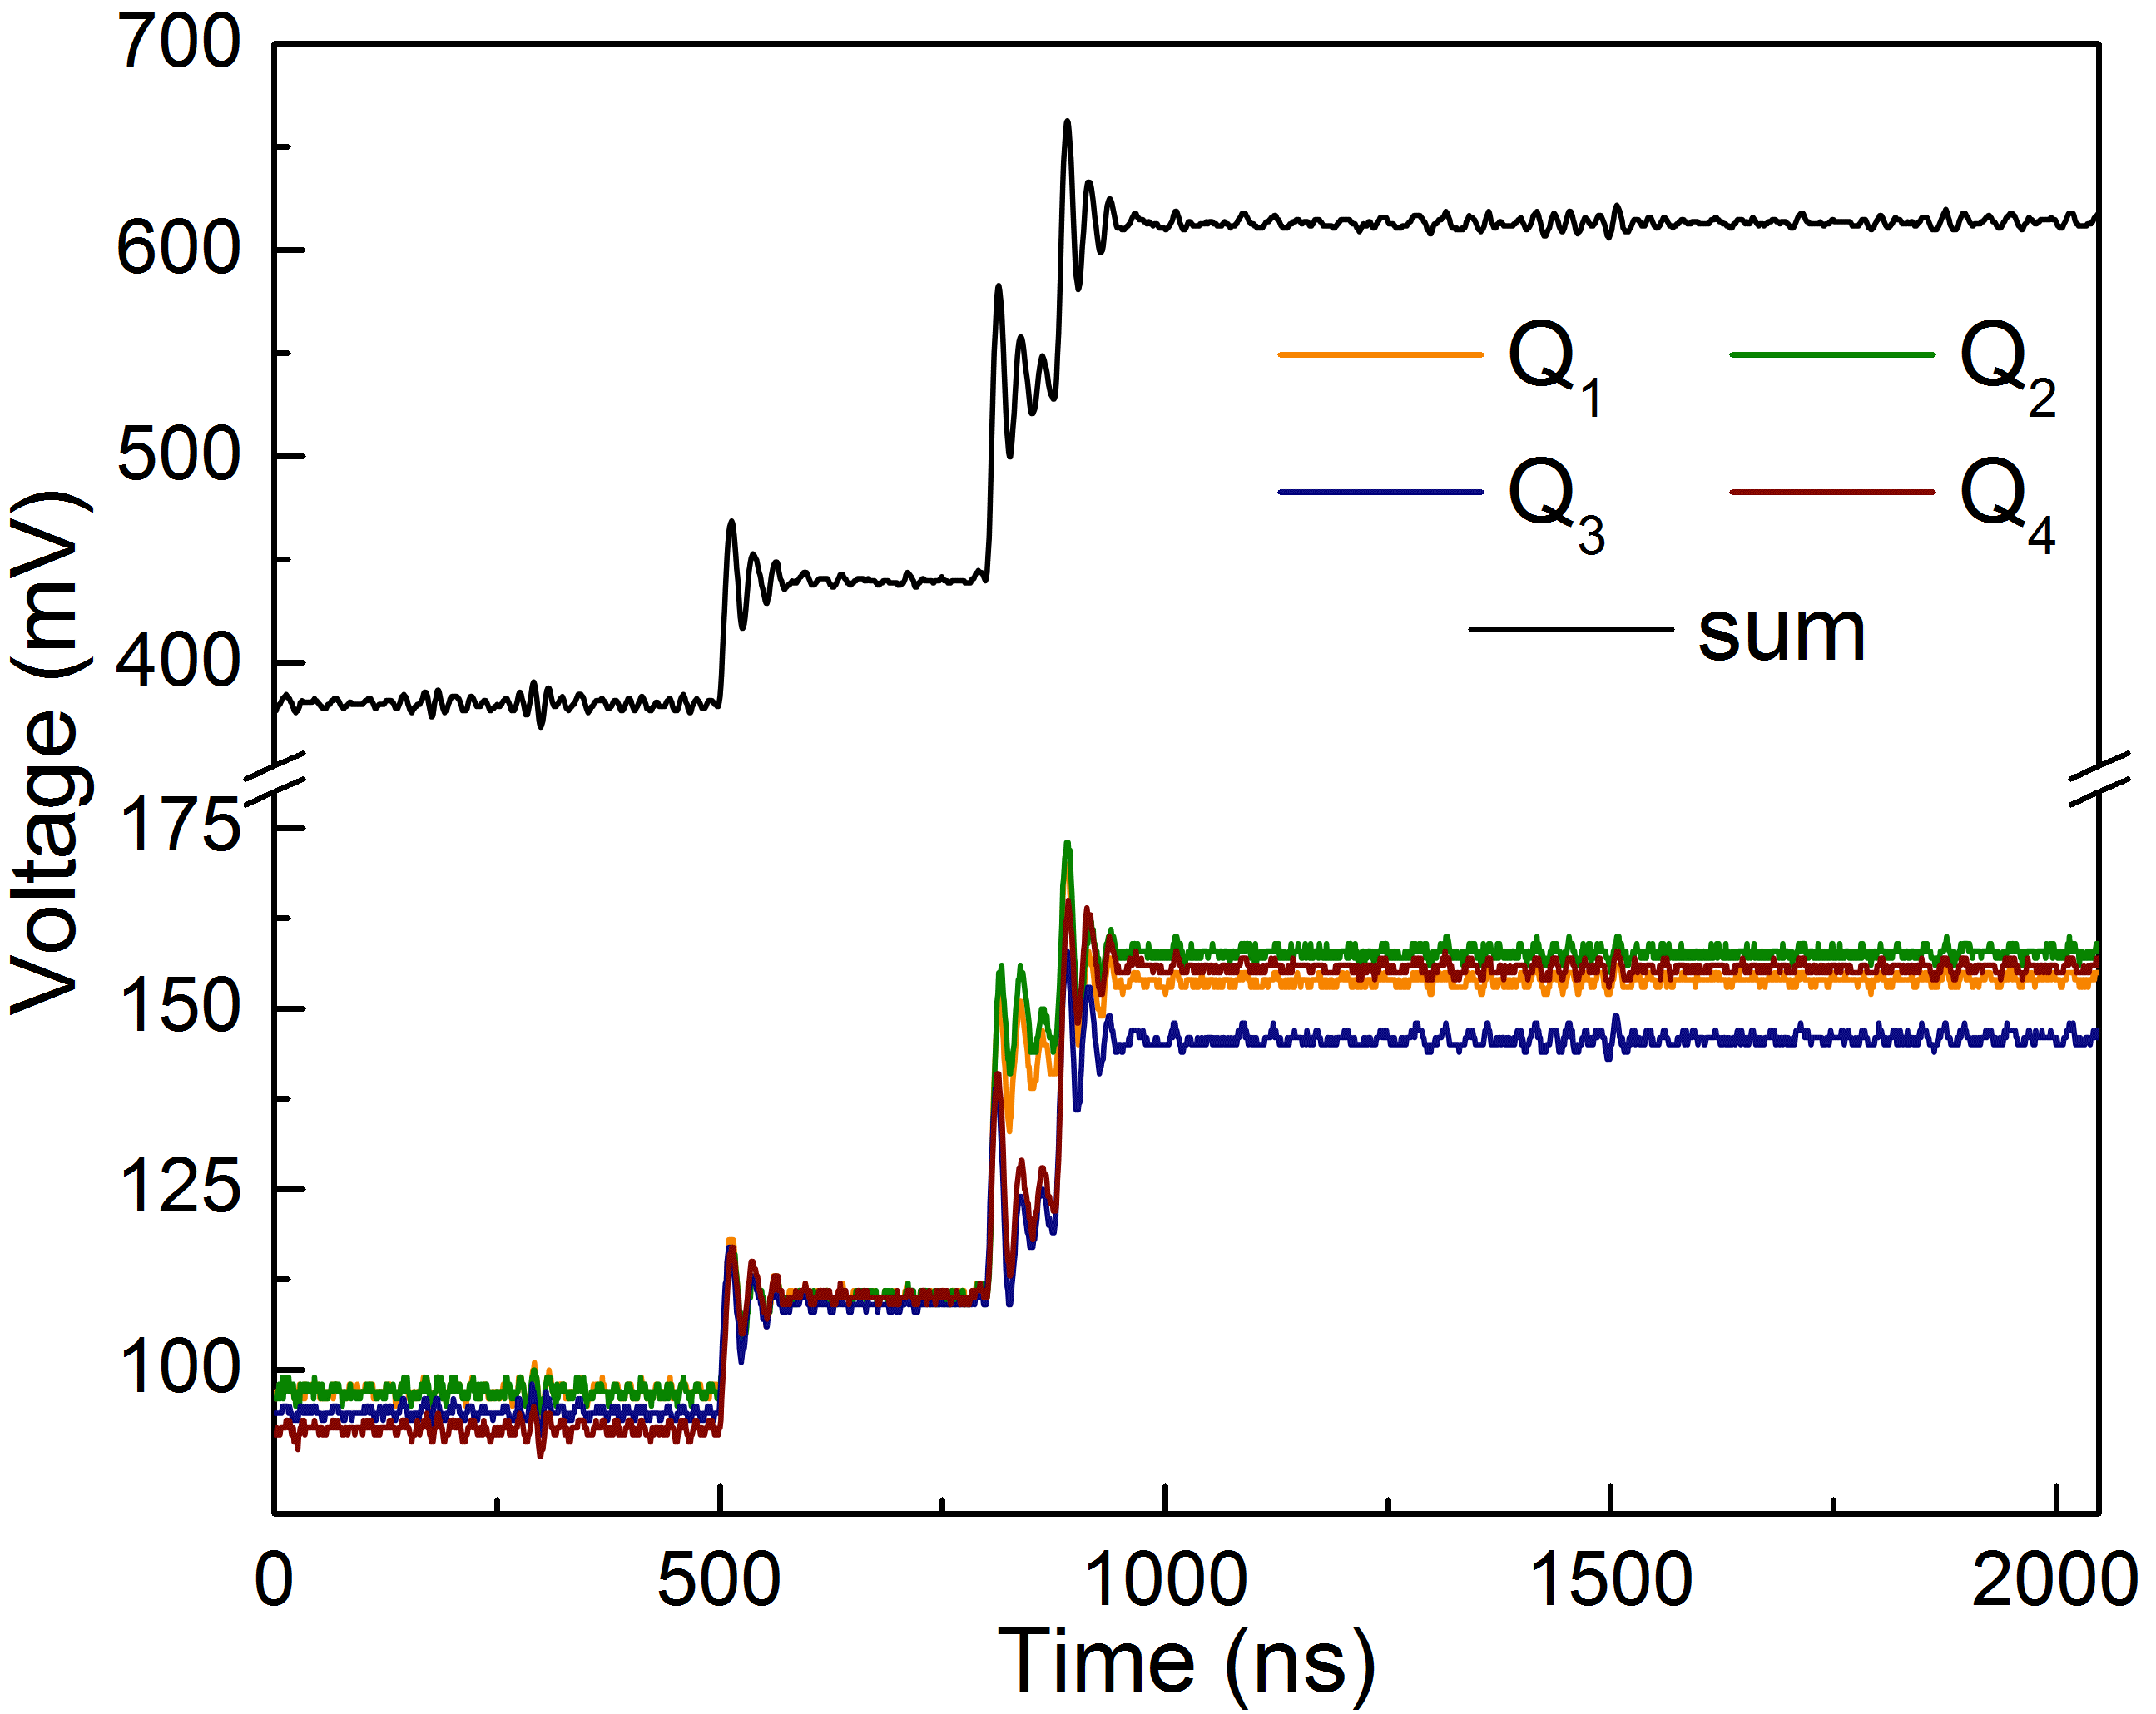
\includegraphics[width=\textwidth]{gfx/TripleCoincidenceEvent}
  \caption
  [Spectrometer response during a triple coincidence event.]
  {Spectrometer response during a triple coincidence event. This was taken during a CEI experiment studying the dynamics of \ch{CS2} at the Canadian Light Source. The fragmentation event showcased is the concerted breakup process \ch{CS2 $\rightarrow$ CS2^3+ $\rightarrow$ C^+ + S^+ + S^+}. As the carbon atom is lighter, the first step at \SI{500}{\ns} is the detection of the carbon atom. All four channels increase by roughly similar amounts hinting that the carbon atom was detected near the center of the detector by \eqref{eq:xy}. Then the second and third events belong to the two sulfur atoms, arriving later due to sulfur's larger atomic mass. If the molecule was aligned in a plane parallel to the detector, the two sulfur atoms would have remained at the same height throughout the Coulomb explosion and been detected at the same time, producing one step in the signal. However, it must have oriented vertically such that one sulfur atom was closer to the detector. During the Coulomb explosion, the closer atom will initially experience a kick towards the detector while the other sulfur atom will initially experience a kick away from the detector before being accelerated upwards due to the constant electric field. This results in one sulfur atom arriving earlier, and the other later. Looking at the individual signals, we see a significant increase in $Q_1$ and $Q_2$ at \SI{800}{\ns} suggesting that the first sulfur atom was on one side of the detector while the more significant increase in $Q_3$ and $Q_4$ at \SI{900}{\ns} suggest that the second sulfur atom was on the other side. This makes some intuitive sense as we expect the carbon atom to land somewhere near the middle and the two sulfurs to land on opposite sides of the detector. The oscilloscope cards sport an 8-bit bus and so the individual $Q_i$ channels were limited to \SI{200}{\mV} to increase position detection accuracy. I must admit that a nice and rich signal such as this one only makes up 1\% of all events, the majority being single or double coincidences.}
  \label{fig:tripleCoincidence}
\end{figure}

Software can analyze the signals and determine the magnitude of each $Q_i$ signal. If the change in baseline before and after an event is denoted $Q_i'$ then the position of the electron is then calculated using
\begin{equation}\label{eq:xy}
x = \frac{Q_1' + Q_2'}
         {Q_1' + Q_2' + Q_3' + Q_4'} ,\quad
y = \frac{Q_1' + Q_3'}
         {Q_1' + Q_2' + Q_3' + Q_4'}
\end{equation}
where $x,y \in [0,1]$ are fractional positions. Multiplying $x$ and $y$ by the dimensions of the MCP detector will yield the physical position of the cloud's centroid.

\subsection{Calculating the atomic fragments' momenta}
Calculating the momentum vector of each atomic fragment is an elementary physics problem once we have the time and position measurements. Let us look at the $p_x$ and $p_y$ components first.

The components of the three-dimensional momentum vector $\mathbf{p} = (p_x,p_y,p_z)$ for each atom are then calculated as

\begin{equation}\label{eq:CEImomenta}
p_x = \frac{m(x-x_0)}{t} ,\;
p_y = \frac{m(y-y_0)}{t} ,\;
p_z = \frac{qV}{2\ell} \left( \frac{t_0^2 - t^2}{t} \right)
\end{equation}
where $m$ is the atom's mass, $(x,y)$ is the location the atom collided with the MCP detector, and $(x_0,y_0)$ is the location that the Coulomb explosion originated. The location $(0,0)$ corresponds to the physical center of the MCP detector. $q$ is the net charge of the atom, $V$ is the value of constant electric potential the atom is subjected to, and $\ell$ is the distance from the location of the Coulomb explosion to the detector. $t$ is measured time of flight (between Coulomb explosion and detection) of the atom and 
\begin{equation}
t_0 = \sqrt{\frac{2d\ell}{V} \left( \frac{m}{q} \right)}
\end{equation}
is the atom's time of flight assuming no external forces act on it during its trip to the detector.

\subsection{Measurement uncertainty in the momenta} \label{ssec:measurementUncertainty}
For any relation $f = f(x_1, x_2, \dots, x_n)$, assuming independent variables (neglecting correlations), the standard deviation (or absolute uncertainty) in a quantity $f$, which we denote $\Delta f$, may be calculated using the variance formula \citep{Ku66}, which has been very popular among physical scientists,
\begin{equation} \label{eq:varianceFormula}
\Delta f = \sqrt{\sum_{i=1}^{n} \left( \frac{\partial f}{\partial x_i} \Delta x_i \right)^2}
\end{equation}
where $\Delta x_i$ is the standard deviation in the independent variable $x_i$ and where the partial derivatives $\partial f/\partial x_i$ are evaluated at the mean of $x_i$. This formula relies on the linear characteristic of the gradient of $f$ and so it's a good estimate for the standard deviation of $f$ as long as the standard deviations $\Delta x_i$ are small compared to the partial derivatives. As it employs a truncated Taylor series, it may even be a biased estimate in some cases. Much can be said about which formula to use in the propagation of uncertainty, and expository articles on the subject have been written by \citet{Birge39} and \citet{Ku1966}, the latter of which provides a derivation of \eqref{eq:varianceFormula}. In our case, we will not attempt to make accurate nor precise calculations of any uncertainty, so we will not fuss about which method we choose to propagate our uncertainties forward. We are simply interested in making rough estimates of the uncertainties on the measured momentum vectors to make rough estimates on the uncertainty of reconstructed geometries in chapter \ref{ch:uncertainty}.

Using \eqref{eq:varianceFormula} we may calculate the uncertainty in the measured momentum values, which will we different for each component. In our case, $p_x = p_x(m,x,x_0,t)$ and $p_y = p_y(m,y,y_0,t)$, however, the uncertainty in the atomic mass $m$ is orders of magnitude smaller than the uncertainty in the other variables and so we will ignore its effects. Thus we get that
\begin{subequations}
  \begin{align}
  \Delta p_x &= \sqrt{
    \left( \frac{\partial p_x}{\partial x}\Delta x \right)^2
    + \left( \frac{\partial p_x}{\partial x_0}\Delta x_0 \right)^2
    + \left(\frac{\partial p_x}{\partial t}\Delta t \right)^2
   } \\
  \Delta p_y &= \sqrt{
    \left( \frac{\partial p_y}{\partial y}\Delta y \right)^2
    + \left(\frac{\partial p_y}{\partial y_0}\Delta y_0 \right)^2
    + \left(\frac{\partial p_y}{\partial t}\Delta t \right)^2
  }
  \end{align}
\end{subequations}
where the partial derivatives can be calculated from \eqref{eq:CEImomenta} as
\begin{subequations}
  \begin{align}
  \frac{\partial p_x}{\partial x} = \frac{m}{t} &,\quad \frac{\partial p_x}{\partial x_0} = \frac{m}{t} ,\quad \frac{\partial p_x}{\partial t} = -m\frac{x-x_0}{t^2}\\
  \frac{\partial p_y}{\partial y} = \frac{m}{t} &,\quad \frac{\partial p_y}{\partial y_0} = \frac{m}{t} ,\quad \frac{\partial p_y}{\partial t} = -m\frac{y-y_0}{t^2}
  \end{align}
\end{subequations}
and so
\begin{subequations}
  \begin{align}
  \Delta p_x &= p_x \sqrt{
    \left( \frac{\Delta x}{x - x_0} \right)^2
    + \left( \frac{\Delta x_0}{x - x_0} \right)^2
    + \left( \frac{\Delta t}{t} \right)^2 } \\
  \Delta p_y &= p_y \sqrt{
    \left( \frac{\Delta y}{y - y_0} \right)^2
    + \left( \frac{\Delta y_0}{y - y_0} \right)^2
    + \left( \frac{\Delta t}{t} \right)^2 }
  \end{align}
\end{subequations}

Repeating the process for $p_z = p_z(q,V,\ell,t_0,t)$ but ignoring the tiny uncertainties in $q$, $V$, and $\ell$, we get
\begin{equation}
\Delta p_z = p_z \sqrt{
  \left( \frac{2tt_0}{t_0^2 - t^2} \Delta t_0 \right)^2
  + \left( \frac{t^2 + t_0^2}{t(t_0^2 - t^2)} \Delta t^2 \right)^2
}
\end{equation}

\section{Exploratory data analysis}
Before we attempt to reconstruct geometries based on the momentum vectors measured, it would be a good idea to inspect and analyze the raw data first. Such an analysis will help us identify any issues with the data and really we should be making sense of the raw data before attempting to analyze it further. Such an analysis is typically termed exploratory data analysis, first promoted by \citet{Tukey77}.

For each Coulomb explosion event, our measurements for \ch{OCS} include a momentum vector $(p_x, p_y, p_z)$ for each atom or fragment. Thus each event involves the measurement of $9$ scalars, ultimately forming a $9$-dimensional multivariate dataset with some structure, mainly imposed by the condition that momentum must be conserved along each physical axis in the reference frame of the molecule, that is the center-of-momentum (COM) frame for us.

For this section we will look at the momentum vectors measured for \ch{OCS} in the $(2,2,2)$ fragmentation channel following Coulomb explosion by a \SI{7}{\fs} laser pulse, with all measurements kept in the lab frame. This allows us to inspect the raw data before it is transformed to the COM frame with the added benefit that it allows for the inspection of any instrumental or systematic errors. Qualitatively, the data looks quite similar in the two frames, but the geometry reconstruction can only be done in the COM frame as the simulation assumes that the molecule starts from rest such that momentum is always conserved as the molecular systems undergoes a Coulomb explosion.

In figure \ref{fig:OCS2227fsMomentum} we plot histograms for each atom's momentum components and overlay the histograms with kernel density estimates (using a Gaussian kernel) to estimate the probability density function of each momentum component. Glancing at the distributions, they seem to make sense qualitatively with some pecularities as discussed in the caption. 

This analysis should be done for each data set collected. So for us, it should be repeated for the 30, 60, 100, and \SI{200}{\fs} data sets which we include in appendix \ref{appx:supplementaryFigures} as figures \ref{fig:OCS22230fsMomentum}--\ref{fig:OCS222200fsMomentum}.

\begin{figure}
  \centering
  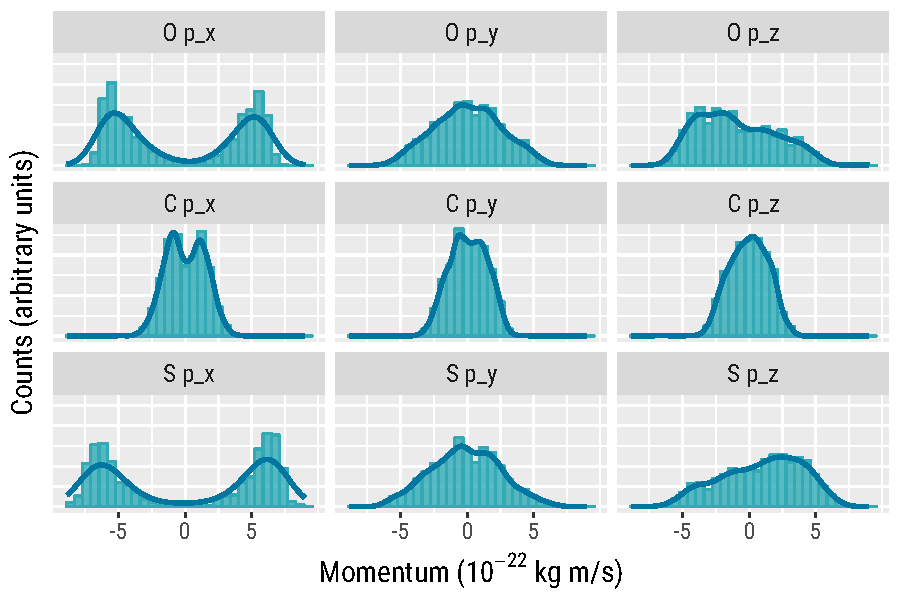
\includegraphics[width=\textwidth]{Plots/OCS2227fsMomentum}
  \caption[Distributions for each atom's momentum components measured after Coulomb explosion by a \SI{7}{\fs} laser pulse for the $(2,2,2)$ fragmentation channel (in the lab frame).]
  {Distributions for each atom's momentum components measured after Coulomb explosion by a \SI{7}{\fs} laser pulse for the $(2,2,2)$ fragmentation channel (in the lab frame). We can infer some basic dynamics from these plots. For example, we see that the oxygen and sulfur atoms tend to fly off with high velocity in the $x$-direction while the carbon atom flies off with little velocity in the $x$-direction. As conversation of momentum must hold, the $p_x$ component of the molecular system must sum to zero suggesting that the oxygen and sulfur tend to fly off in opposite $x$-directions. This is expected as they are both terminal atoms and confirms that the data makes physical sense. The other distributions do not say much except for the slight asymmetry in the oxygen and sulfur's $p_z$ distributions which may be due to instrumental bias in measuring the arrival time of atomic fragments. We also notice that the momentum distribution is rather isotropic in the $y$ and $z$ directions but is bimodal in the $x$ direction, suggesting that the laser pulse's electric field was polarized along the $x$-axis. Kernel density estimates (with a Gaussian kernel) are used to estimate the probability density function of each momentum component. Such estimates are inherently not as effective at estimating bimodal distributions thus the carbon and sulfur's $p_x$ estimates appear oversmoothed. To inspect this 9-dimensional distribution in more detail we look to figure \ref{fig:OCS2227fsMomentumPairPlots}.}
  \label{fig:OCS2227fsMomentum}
\end{figure}

While figure \ref{fig:OCS2227fsMomentum} gives us some insight into the measurements, we are looking at a multidimensional data set and might want to look at correlations between each measurement. We do this using a pairs plot, which is a grid of scatterplots showing the bivariate relationships between all pairs of variables in a multivariate dataset. The pairs plot was first introduced by \citet{Hartigan75}, however we use the more modern and generalized version introduced by \citet{Emerson13} as they provide an open-source implementation in the form of an R package.

Figure \ref{fig:OCS2227fsMomentumPairPlots} uses a pairs plot to showcase the relationship between ever pair of variables in our dataset. Due to the $9$-dimensional nature of our dataset, we end up with a $9\times9$ grid of plots with some redundancy. The diagonal repeats the kernel density estimates shown in figure \ref{fig:OCS2227fsMomentum} but they are quite useful as a reference here. Below the diagonal are the scatter plots, however due to the high density of points, contour plots are employed to showcase the same relationship above the diagonal. So only 36 scatter plots are required but this format provides us with greater insight of our dataset.

\begin{figure}
  \centering
  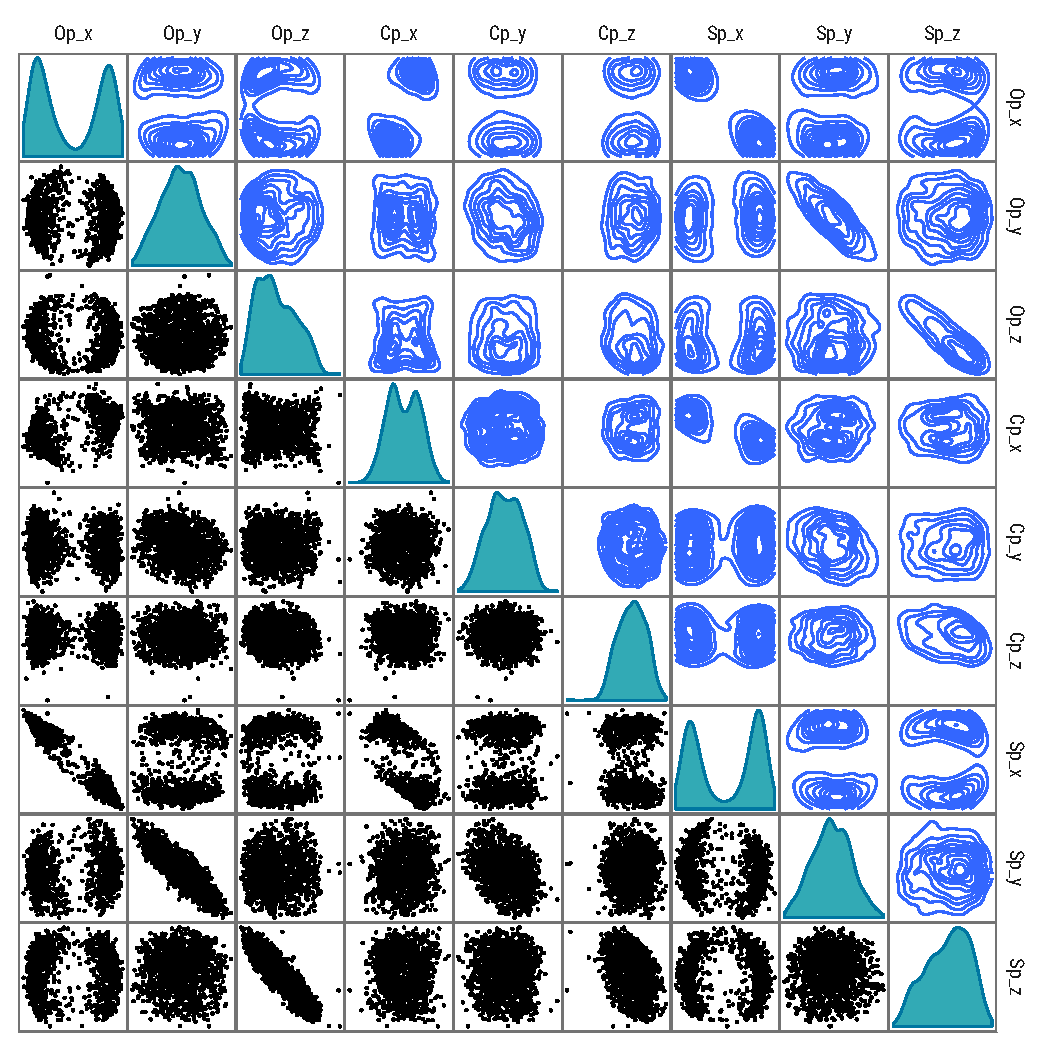
\includegraphics[width=\textwidth]{Plots/OCS2227fsMomentumPairsPlot}
  \caption[Pairs plot showing the bivariate relationship between each atom's momentum components measured after Coulomb explosion by a \SI{7}{\fs} laser pulse for the $(2,2,2)$ fragmentation channel.]
  {Pairs plot showing the bivariate relationship between each atom's momentum components measured after Coulomb explosion by a \SI{7}{\fs} laser pulse for the $(2,2,2)$ fragmentation channel. On the diagonal, kernel density estimates (with a Gaussian kernel) of the momentum component designated by the label at the top of the column and end of the row are given. Below the diagonal, scatter plots show the relationship between the momentum components belonging to that row and column. Above the diagonal, the same relationship is given using a contour plot instead. For example, the scatter plot in row $7$, column $1$ plots the oxygens's $p_x$ component on the $x$-axis and the sulfur's $p_x$ component on the $y$-axis. The contour plot in row $1$, column $7$ shows the same relationship. We see a negative correlation between oxygen's $p_x$ and sulfur's $p_x$ as predicted in figure \ref{fig:OCS2227fsMomentum}'s caption. Similarly we see negative correlations between oxygen's $p_y$ and sulfur's $p_y$ as well as between oxygen's $p_z$ and sulfur's $p_z$, which makes physical sense due to the two atoms being terminal atoms, so they should fly off in approximately opposite directions following a Coulomb explosion.}
  \label{fig:OCS2227fsMomentumPairPlots}
\end{figure}

Pairs plots for the 30, 60, 100, and \SI{200}{\fs} data sets are included in appendix \ref{appx:supplementaryFigures} as figures \ref{fig:OCS22230fsMomentumPairPlots}--\ref{fig:OCS222200fsMomentumPairPlots}.

\section{Computationally simulating a Coulomb explosion} \label{sec:simulating}
To simulate a Coulomb explosion of a molecule containing $n$ atoms, we will make some simplifying assumptions to arrive at the simplest simulation possible simulation that will allow us to investigate the problem of reconstructing geometries. We will assume that the motion of the ions are governed only by their mutual Coulomb repulsion. So we are in effect also assuming that the chemical bonds are broken at $t = 0$ and have no effect on the trajectories of the ions, and that neutral fragments do not interact with any other fragment. We model each atom as a point particle with a fixed  electric charge assigned at $t = 0$ so no charge redistribution can occur. We assume that the atoms each begin at rest at $t = 0$ and that their initial positions are determined by the molecule's equilibrium or ground-state geometry. Of course, these assumptions force us to ignore the rearrangement of the atoms under the influence of the laser pulse's intense electromagnetic field, and any initial momentum imparted on the atoms by this interaction.

Under such assumptions, we can solve the classical equations of motion for each ion right after the explosion. We choose to use Hamiltonian mechanics to acquire a system of $6n$ first-order ordinary differential equations (ODE's) which may be easily solved by numerical methods such as the ubiquitous fourth-order Runge-Kutta. If Lagrangian mechanics is used, then the resulting second-order must be recast as a system of first-order ODE's as numerical algorithms are developed to solve systems of first-order ODE's. The Hamiltonian of the molecular system is
\begin{equation}
\mathcal{H}(\mathbf{r}_i, \mathbf{p}_i, t) = \sum_{i=1}^n \frac{\mathbf{p}_i^2}{2m_i} + \frac{1}{4\pi\epsilon_0}\sum_{\substack{\lbrace i,j\rbrace\\ i \ne j}} \frac{q_iq_j}{|\mathbf{r}_i-\mathbf{r}_j|}
\end{equation}
where $i,j \in \lbrace 1,2,\dots, n \rbrace$ and so the second summation is over all $i,j$ pairs where $i \ne j$. Calculating Hamilton's equations for the system, we get
\begin{subequations}
  \begin{align}
  \frac{d\mathbf{r}_i}{dt} &= \frac{\partial \mathcal{H}}{\partial \mathbf{p}_i} = \frac{\mathbf{p}_i}{m_i} \\
  \frac{d\mathbf{p}_i}{dt} &= \frac{\partial \mathcal{H}}{\partial \mathbf{r}_i} = \frac{1}{4\pi\epsilon_0}\sum_{j, \; j \ne i} \frac{\mathbf{r}_i - \mathbf{r}_j}{|\mathbf{r}_i - \mathbf{r}_j|^3}
  \end{align}
\end{subequations}
where $i$ is held fixed over the second summation. With appropriate initial conditions this system of $6n$ scalar first-order ordinary differential equations may be easily solved using, for example, the classical fourth-order Runge-Kutta method for numerically solving ordinary differential equations. The atoms are assumed to be at rest so that $\mathbf{p}_i(t=0) = 0$, while the initial positions, $\mathbf{r}_i(t=0)$, are chosen to correspond to the molecular geometry.

One way to think of the problem being tackled in this thesis is: which initial geometry $\mathbf{r}_i(t=0) = 0$ results in the momentum values measured at the detector? The atoms are far enough apart after just a few nanoseconds that by the time they arrive at the detector, they feel almost no forces due to each other and their momenta attain asymptotic values which we can denote $\mathbf{p}_i(t\rightarrow\infty)$.

\section{Describing geometries and momenta} \label{sec:conventions}
While tackling the problem of geometry reconstruction, it will be crucial to choose a convention for describing the geometries and momentum vectors especially so that geometries and vector arrangements can be compared with ease. Even more importantly, it provides us with an opportunity to reduce the dimensionality of the problem from $3N$ to $3N-6$ for a molecular system with $N$ atoms. This stems from the fact that we only need to describe the relative position of each atom, not its absolute position. For example, a triatomic molecule can be described by two bond lengths and a bond angle, rather than three position vectors. Also, the exact same molecule can produce different momentum vectors after a Coulomb explosion depending on its initial orientation with respect to the detector. We must use a momentum convention to ensure a one-to-one mapping between geometries and measured momentum vectors.

\subsection{Triatomic molecules}
\subsection{Describing larger molecular geometries}
\subsection{Describing momentum vector arrangements}